\chapter{Materiais e Métodos}

\begin{justify}

\hspace{12 mm} Os dados experimentais foram extraídos de projetos prévios e descritos nesse trabalho. A análise das mutações \textit{missense} das variantes de SARS-CoV-2 utilizou-se de abordagens computacionais e dados públicos. As etapas computacionais de coletas das sequências genômicas, identificação das mutações e predição de epitopos  foram baseadas em metodologias prévias \cite{Hamelin:2022}.  


\section{Estudo Experimental}

O município de Foz do Iguaçu, no sul do Brasil, faz fronteira com Paraguai e Argentina. O município tem 258.823 habitantes, uma densidade de 414,58 pessoas por km², urbanização superior a 99\% e um Índice de Desenvolvimento Humano de 0,751. A rede de saúde inclui 36 unidades, sendo quatro hospitais, organizados em cinco distritos. O primeiro caso de COVID-19 foi registrado em 12 de março de 2020, seguido pelo primeiro caso de transmissão local em 25 de março, transmissão comunitária em 7 de abril e o primeiro óbito em 26 de abril.  As medidas de distanciamento social foram iniciadas a partir de 15 de março \cite{Viana:2021}.

Os pacientes COVID-19 positivo admitidos na Unidade de Tratamento Intensivo (UTI), no Hospital Municipal Paulo Germano Lauck, entre 2020 e 2021, foram submetidos à análise genotípica de HLA-B. Os indivíduos foram selecionados priorizando o histórico hospitalar e quadro clínicos melhor documentados durante o período de internação.  A pesquisa fez parte da  Ação 9 de enfrentamento a COVID-19 no âmbito da Universidade Federal da Integração Latino-Americana – Unila, intitulada “Medicina personalizada para tratamento de pacientes COVID-19 em Foz do Iguaçu” (PORTARIA No 193/2020/GR) (ProjCOVID).

\section{Aspectos Éticos}

Essa etapa faz parte do projeto "Perfil da população do oeste paranaense acometido de Síndrome Respiratória Aguda Grave entre 2020 a 2022", aprovado pelo Comitê de Ética em Pesquisa Envolvendo Seres Humanos, CAAE 36189220.3.0000.8527, em 2020,  Número do Parecer: 4.250.900.

\section{Seleção de indivíduos COVID-19 positivo}

As amostras foram coletadas de pacientes admitidos e apresentando testes RT-qPCR positivos anteriormente ou na admissão hospitalar. A coleta foi realizada a partir de julho/2020 à novembro/2020 e maio/2021 à julho/2021. Os pacientes com declaração de nacionalidade estrangeira, tempo de internação no Hospital superior à 65 dias (considerados \textit{outliers}) e que apresentam resultados ambíguos para os genótipos dos grupos alélicos de HLA foram removidos desta análise. 

O histórico hospitalar foi consultado por meio do Sistema de Gestão Tasy (Koninklijke Philips N.V, Inc., Amsterdam, NL) utilizado pelo Hospital Municipal Padre Germano Lauck, assim como, os quadros clínicos atuais foram coletados no projeto ProjCOVID. 

\section{Fase laboratorial}

De cada paciente foram coletados cerca de 6 ml de sangue periférico em tubo contendo anticoagulante EDTA (Tubo Greiner Bio-One) e armazenados em refrigeração - 80$ ͦ^\circ C$ pela equipe de enfermagem hospitalar. As amostras tiveram o DNA extraído via kit extração \textit{Geno Plus Mini} VIOGENE, numerados e armazenados no banco de amostras do LPCM-UNILA . A quantificação de cada amostra foi realizada em espectrofotômetro NanoDrop ND2000 (Thermo Fischer Inc., Waltham, MA, EUA).

Os éxons de HLA classe I \textit{loci} B foram genotipados por Sequenciamento de Grupo Específico (GSSP) via kit   \textit{SeScore Sequencing}  GSSP (One Lamda, Inc), a partir de amostras do DNA extraído dos pacientes SARS-CoV-2 positivo. As amostras foram checadas, purificadas e sequenciadas em sequenciador automático de \textit{DNA ABI 3500} (Thermo Fischer Inc., Waltham, MA, EUA). As análises dos dados obtidos foram realizadas em Software uTYPE Dx HLA \textit{Sequence Analysis} (One Lambda, Inc). Eventualmente algumas amostras apresentaram resultados com ambiguidade em baixo nível de resolução (grupos alélicos), essas amostras foram filtradas. 

\section{Estudo computacional}

Os métodos computacionais buscaram coletar os dados genômicos de variantes que circularam no município de Foz do Iguaçu (Paraná, Brasil) (Figura \ref{fig:fig5}A e \ref{fig:fig5}B), identificação de mutações missense (Figura \ref{fig:fig5}C e \ref{fig:fig5}D), predição da afinidade de ligação de peptídeos virais mutados (Figura \ref{fig:fig5}E e \ref{fig:fig5}F) e análise descritiva e estatística (Figura \ref{fig:fig5}G). Além disso, dados experimentais de projetos anteriores foram utilizados para direcionar a escolha dos alelos HLA-B selecionados neste estudo.

\begin{wrapfigure}{c}{\textwidth}
    \centering
    \caption{\justifying Etapas do \textit{pipeline} para análise das mutações \textit{missense}. Coletas de dados genômicos (A), alinhamento das sequências das mesmas variantes (B), alinhamento das sequências consenso de cada variante com a sequência de referência (C), identificação de mutações \textit{missense} (D), geração dos peptídeos de referência e mutados (E), predição da afinidade de ligação (F) e análise estatística (G). Quadros vermelhos apresentam dados quantitativos de cada etapa. }
    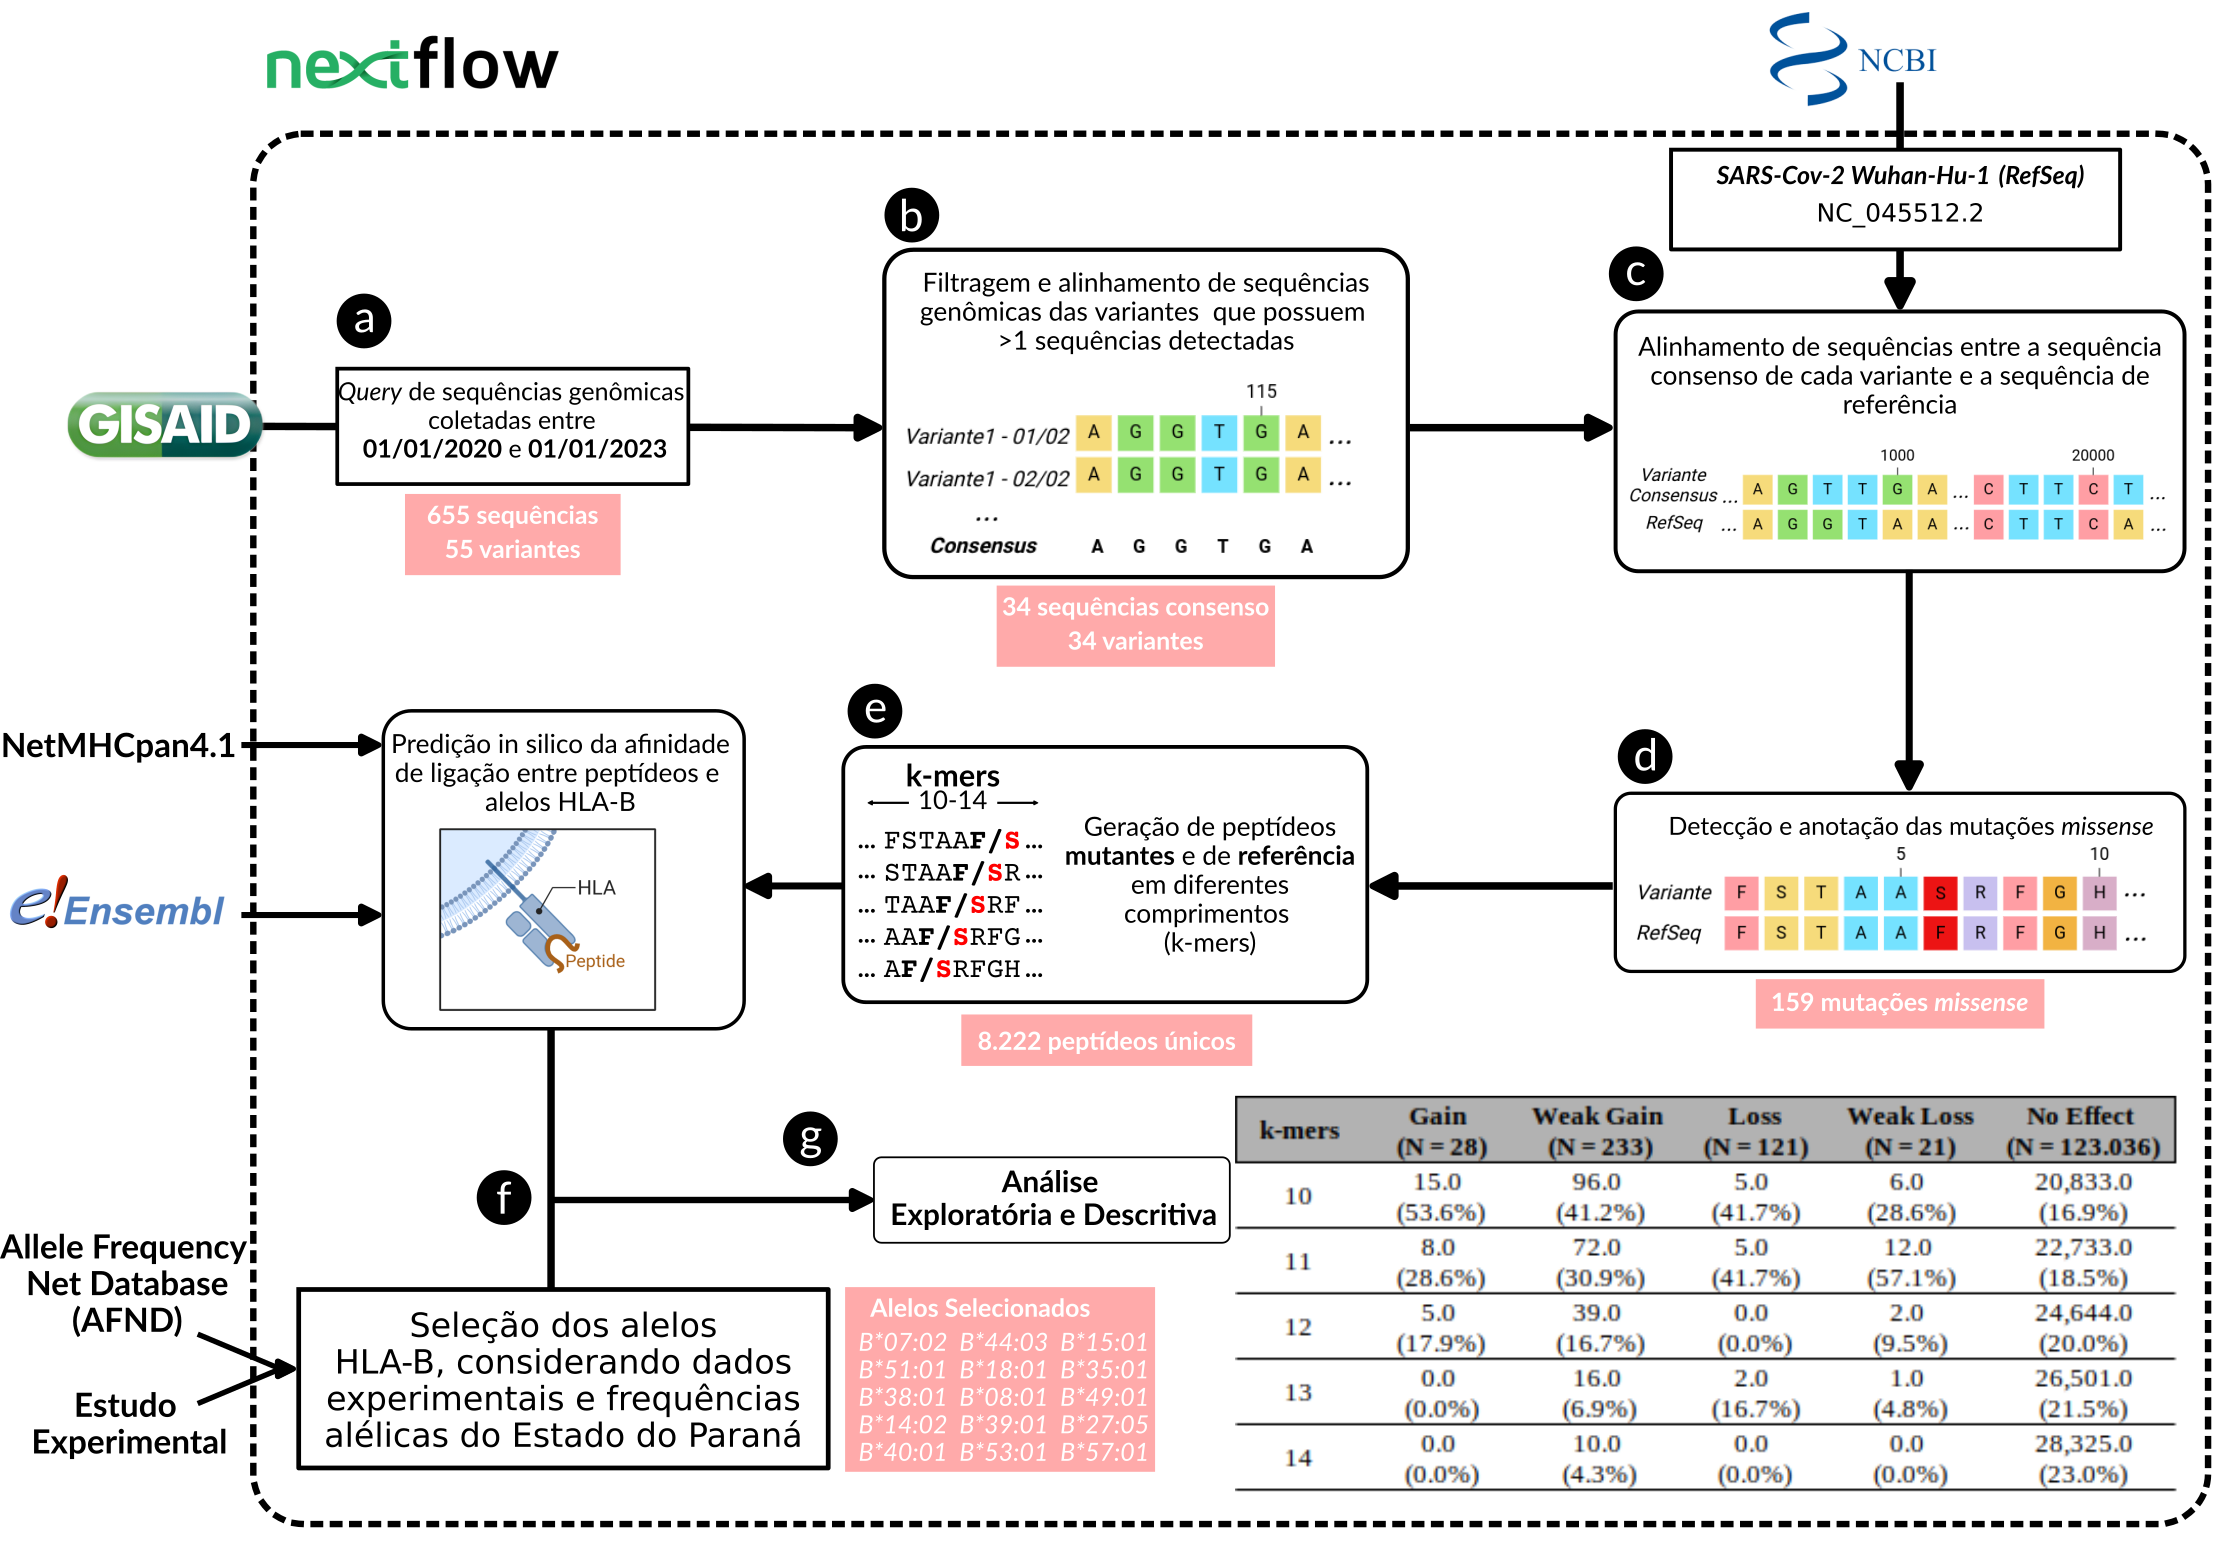
\includegraphics[width=1\textwidth]{Figuras/fig5.png}
    \label{fig:fig5}
    \begin{minipage}{0.8\textwidth} % Adjust width as needed
        \centering
        \footnotesize Fonte: O Autor (2024)
    \end{minipage}
\end{wrapfigure}

\begin{wrapfigure}{c}{0pt}
\end{wrapfigure}

\section{Coleta de dados genômicos}

As 655 sequências genômicas de SARS-CoV-2 foram coletadas via GISAIDR (versão 0.9.10) \cite{Wirth:2022} a partir do banco de dados EpiCoV, pertencente ao \textit{Global Initiative on Sharing All Influenza Data} (GISAID) \cite{Khare:2021}. A requisição foi realizada para sequências genômicas completas ($\geq$29kb) coletadas entre 01/01/2020 e 01/01/2023, extraídas a partir de amostras provenientes da cidade de Foz do Iguaçu - Paraná/Brasil (Figura \ref{fig:fig5}A e \ref{fig:fig5}B). As 55 variantes detectadas foram inferidas com base na classificação fornecida pelo \textit{EpiCoV}. Sequências com mais de 5\% das bases desconhecidas, extraídas de amostras ambientais ou variantes que tiveram apenas uma sequência coletada foram excluídas. O banco de sequências utilizado neste estudo pode ser acessado via
 \href{http://gisaid.org/EPI_SET_240517bd}{gisaid.org/EPI\_SET\_240517bd}.

\section{Identificação de mutações \textit{missense} de SARS-CoV-2}

As sequências consenso foram obtidas a partir de sequências alinhadas de mesma variante. A sequência de referência SARS-CoV-2 Wuhan-1 (NC\_045512.2) foi alinhada com cada sequência consenso individualmente utilizando \textit{minimap2 v2.26-r1175}. As sequências mapeadas foram  ordenadas e convertidas em um arquivo \textit{.bam} utilizando \textit{samtools v1.18}. A chamada das variantes foi realizada utilizando \textit{bcftools mpileup v1.17} no modo haplóide e mutações somáticas foram anotadas a partir de \textit{snpEff v4.3} com a função \textit{ann} (Figura \ref{fig:fig5}D).

\section{Predição da afinidade de ligação de peptídeos virais mutados}

Os peptídeos virais foram selecionados a partir da posição de mutação, gerando \textit{k-mers} de 10 à 14 aminoácidos com a presença de mutação única em cada uma das posições, assim como, peptídeos não mutados como referência (Figura \ref{fig:fig5}E). Os peptídeos que apresentavam similaridade e identidade completa com peptídeos do genoma humano \textit{GRCh38} foram descartados utilizando o \textit{Ensembl BioMart} \cite{Harrison:2024, Kinsella:2011}. A afinidade de ligação dos peptídeos virais selecionados foi predita contra 15 alelos de HLA-B (B*07:02, B*08:01, B*14:02, B*15:01, B*18:01, B*27:05, B*35:01, B*38:01, B*39:01, B*40:01, B*44:03,  B*49:01,  B*51:01, B*53:01, B*57:01). A escolha dos alelos teve como base os grupos alélicos presentes nas coletas experimentais realizadas em 2020  e 2021 pelo laboratório, além de acrescentar alelos frequentes no Estado Paraná detectados no Registro Brasileiro de Doadores Voluntários de Medula Óssea (REDOME) e em estudos prévios (Apêndice A).

A predição da afinidade de ligação dos peptídeos foi realizada pelo NetMHCpan 4.1 EL, esse método utiliza uma rede neural treinada com dados experimentais de afinidade de ligação e dados de ligantes eluídos para gerar uma pontuação que indica a probabilidade de um peptídeo ser um ligante para os tipos de HLA especificados \cite{Reynisson:2020}. A probabilidade de ligação é expressa em forma de classificação percentílica (\%rank), onde os ligantes classificados como fracos (\textit{Weak binder}, WB) obtiveram um \%rank abaixo de 2.0, enquanto os ligantes fortes (\textit{Strong binder}, SB) obtiveram um \%rank abaixo de 0.5 ou não ligantes (\textit{Non binder}, NB) obtêm um \%rank acima de 2.0 (Figura \ref{fig:fig5}E). 

Com base nesse sistema de classificação, os pares de peptídeos referência/mutados que apresentaram uma transição de classificação a partir das mutações foram reclassificados com base na perda ou ganho de afinidade de ligação. As mutações que fizeram peptídeos passar de ligantes fortes (SB) para ligantes fracos (WB) ou não-ligantes (NB) levam a classificação de uma leve perda (Weak loss) ou uma perda de ligação (Loss), respectivamente. Enquanto que mutações que causam um ganho de afinidade de ligação de WB para SB ou de NB para SB foram consideradas como um leve ganho de ligação \textit{Weak gain} ou \textit{Gain}, respectivamente (Figura \ref{fig:fig5}F e \ref{fig:fig6}).

\begin{wrapfigure}{c}{\textwidth}
    \centering
    \caption{\justifying Esquema demonstrando o conceito de perda (\textit{Loss}) e ganho (\textit{Gain}) de afinidade de ligação dos epítopos de referência e mutados. }
    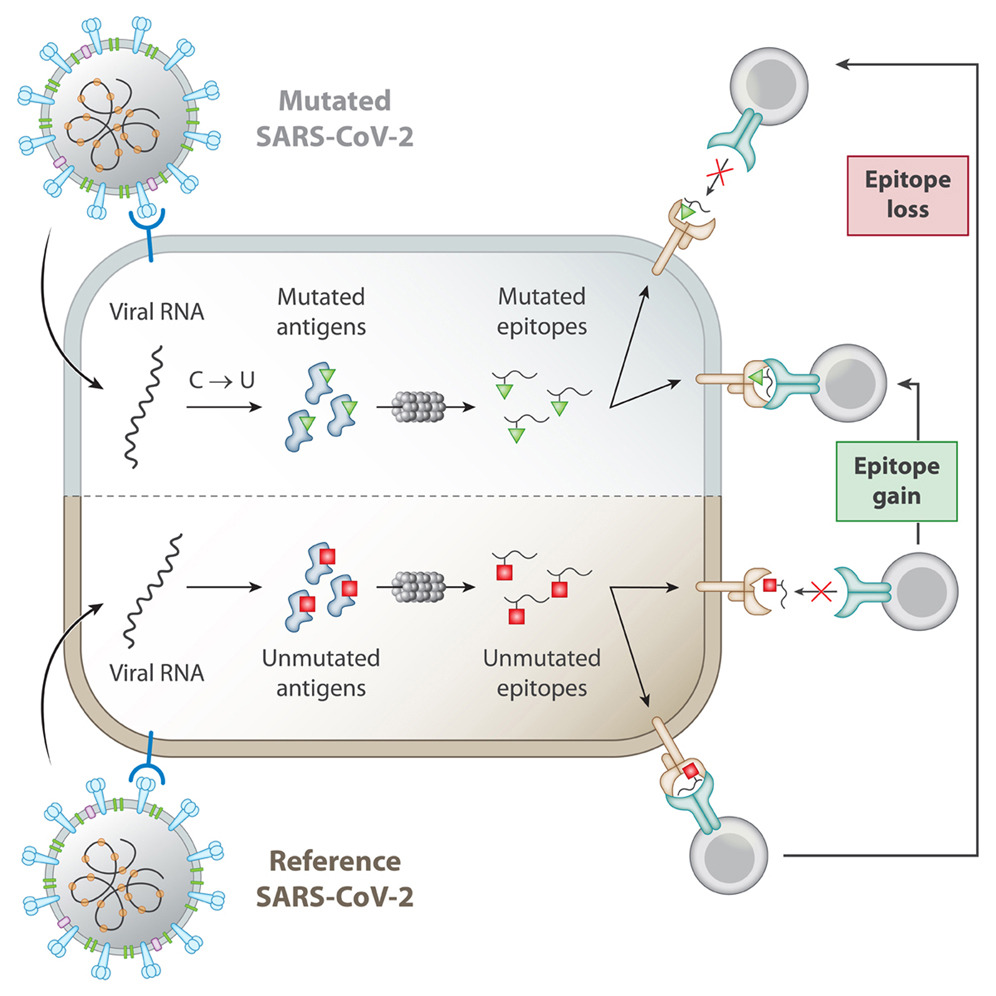
\includegraphics[width=0.7\textwidth]{Figuras/fig6.jpg}
    \label{fig:fig6}
    \begin{minipage}{0.8\textwidth} % Adjust width as needed
        \centering
        \footnotesize Fonte: \citeonline{Hamelin:2022}
    \end{minipage}
\end{wrapfigure}

\begin{wrapfigure}{c}{0pt}
\end{wrapfigure}

\section{Análise estatística}

O teste não-paramétrico de Sinais de Wilcoxon foi aplicado para definir a significância estatística entre os valores de \%rank para peptídeos de referência e mutantes em relação a cada alelo analisado (Figura \ref{fig:fig5}F). A amplitude de impacto de cada mutação que gerou perda na afinidade de ligação foi analisada por meio da equação \eqref{eq:fc}, transformação \textit{log} a partir do valor de \%rank com mutação normalizado em relação ao \%rank de referência:
%

\begin{subequations}
\begin{gather}

\log_2(Fold\;Change) = \log_2(\dfrac{\%rank_{mutação}}{\%rank_{referência}})   \label{eq:fc} 

\end{gather}
\end{subequations}


Os grupos alélicos detectados no Estudo Experimental foram organizados pela data de admissão hospitalar e grupos alélicos que foram detectados em menos de 10 pacientes, entre 2020 e 2021, foram agrupados em "Outros". Os p-valores das comparações das frequências de HLA-B entre os grupos foram obtidos por Teste Exato de Fisher ao nível de significância adotado de 5\% (\( p < 0.5 \)). Quando mencionado, os p-valores foram ajustados para múltiplas comparações com o método de Bonferroni. 

\section{Modelo Estrutural}

O modelo estrutural da glicoproteína spike (na forma clivada no sítio de clivagem da furina) com uma ligação ao ACE2 foi utilizado a partir dos conjuntos de coordenadas do PDB ID:7A94 \cite{Benton:2020}. O software Pymol (The PyMOL Molecular Graphics System, v.2.2.0) foi empregado para visualização.

\section{Ferramentas Computacionais}

O \textit{pipeline} foi construído com Nextflow v23.10.1.5891 e as diferentes etapas para predição da afinidade de ligação foram executadas via Python 3.10, utilizando um script adaptado a partir do \textit{pipeline nf-core/epitopeprediction v2.2.1} \cite{Mohr:2024}.  As análises de dados e gráficos foram produzidos no software RStudio v2023.06.02 (R versão 4.4). Os códigos e os dados estão disponíveis em \href{https://github.com/chagas98/sarscovHLAFoz}{github.com/chagas98/sarscovHLAFoz}.

\end{justify}